\documentclass[12pt]{report}
\usepackage[table,xcdraw]{xcolor}
\usepackage[T1]{fontenc}
\usepackage[utf8]{inputenc}
\usepackage{lmodern} % Or another pdflatex-compatible font package
\usepackage{amsmath, amsfonts, amssymb}
\usepackage{graphicx}
\usepackage{hyperref}
\usepackage{geometry}
\usepackage{physics}
\usepackage{fancyhdr}
\usepackage{tikz}
\usepackage{listings}
\usepackage{xcolor}
\usepackage{amssymb}
\usepackage{float}
\usepackage{subcaption}
\usepackage{amsthm} % Enables theorems, lemmas, etc.
\usepackage[framemethod=tikz]{mdframed}
\usepackage{yfonts}
\usepackage{physics}
\geometry{margin=1in}
\usepackage[backend=biber,style=numeric,defernumbers=true]{biblatex}
\addbibresource{chapter1_citationsfull.bib}
\mdfdefinestyle{collapsebox}{
  linecolor=black,
  outerlinewidth=1pt,
  roundcorner=8pt,
  innertopmargin=10pt,
  innerbottommargin=10pt,
  backgroundcolor=black!3,
  nobreak=true
}

\newtheorem{theorem}{Theorem}[section] % Theorem numbering per section


\lstset{
  language=Python,
  basicstyle=\ttfamily\footnotesize,
  breaklines=true,
  breakatwhitespace=true,
  frame=single,
  columns=flexible,
  keepspaces=true,
  numbers=left,
  numberstyle=\tiny\color{gray},
  stepnumber=1,
  numbersep=5pt,
  tabsize=4,
  showstringspaces=false,
  keywordstyle=\color{blue},
  commentstyle=\color{gray!70!black}\itshape,
  stringstyle=\color{orange},
  backgroundcolor=\color{black!1},
  rulecolor=\color{black!40},
}


\setlength{\headheight}{15pt} % or higher if needed
\addtolength{\topmargin}{-3pt} % to balance page layout
\geometry{margin=1in}

\title{Measurement: A Reconciliation}
\author{Ryan Luke Russell}
\date{\today}
\usepackage{eso-pic}


\newcommand\BackgroundPic{%
  \AddToShipoutPictureBG*{%
    \ifnum\value{page}>1
      \begin{tikzpicture}[remember picture,overlay]
        \node[opacity=0.2, at=(current page.center)] {
          
\includegraphics[width=0.8\paperwidth]{images/morningstar.png}
        };
      \end{tikzpicture}
    \fi
  } 
}



\begin{document}
% Fancy header/footer
\pagestyle{fancy}
\fancyhf{}
\lhead{\leftmark}
\rhead{\thepage}
\renewcommand{\headrulewidth}{0.4pt}
\renewcommand{\footrulewidth}{0pt}



\begin{titlepage}
    \centering
    \vspace*{2.5cm}
    {\Huge\bfseries Measurement: A Reconciliation \\[0.5em]}
    {\LARGE Ryan Luke Russell}\\[0.5cm]
    {\large \today}\\[3cm]
    
\includegraphics[width=0.4\textwidth]{images/morningstar.png}\\[1cm]
    {\Large\itshape \textquotedblleft Photizein tous agnoountas\textquotedblright}\\
    {\large - PHOTIZARE IGNORANTES}
    \vfill
\end{titlepage}

\begin{abstract}
The divide between quantum indeterminacy and classical structure remains one of the most persistent foundational problems in physics. This work proposes a novel field-theoretic framework in which measurement is reinterpreted not as an external trigger but as a fundamental physical field, one that propagates, accumulates, and induces definitional collapse. Building on a mathematical foundation involving imaginary matrices and Euler's identity as a collapse operator, we model the emergence of classical reality as a gradient-driven field transition. This Measurement Field Theory (MFT) treats observation as a dynamical interaction with quantifiable consequences, allowing collapse to be expressed in terms of spatial curvature, thermodynamic entropy, and non-local field behavior. We derive evolution equations, propose experimental predictions, and demonstrate how measurement fields may unify the mechanisms underlying decoherence, virtual particle emergence, phase transitions, and even dark matter phenomena. This framework aims to bridge the quantum-classical interface by treating definition itself as a propagating force, not metaphorically, but as a measurable and testable entity in field-theoretic terms.
\end{abstract}
  
\tableofcontents

\chapter{Measurement: A Reconciliation}

\section{Introduction: The Case for Measurement as a Physical Field}

Classical physics and quantum mechanics diverge sharply in their treatment of measurement, stability, and state definition. In this work, we propose a unifying formalism based on imaginary matrices, Euler's identity as a collapse operator, and field-theoretic constructions of measurement dynamics. Through this framework, the transition from probabilistic phase spaces to resolved realspace structures is modeled as an observable and quantifiable physical process.

The fundamental assertion of this work is that measurement itself constitutes a physical field-one that exists on a gradient, propagates over space and time, and exerts force-like influence on systems. This directly challenges the Copenhagen interpretation (measurement as binary or observer-triggered) and extends collapse dynamics into a field-theoretic, testable framework. As we shall demonstrate, there is only one known mechanism of collapse-and that is measurement, not conscious thought, but measurement as a physical act.

\section{Euler's Identity as the Fundamental Collapse Operator}

\begin{flushright}
  {\itshape "When possibility coils upon itself, the very act of looking forces it to snap."}
\end{flushright}

At the heart of Measurement Field Theory (MFT) lies a brutal truth: the universe does not reveal itself until it is forced to. This forcing-\emph{collapse}-is captured by the simplest, yet most profound of equations:

\begin{equation}\label{eq:euler}
  e^{i\pi} = -1
\end{equation}

Euler's identity is not a cute mathematical trick. It is the \emph{fingerprint of reality's selection mechanism} \cite{gothen_eulers_2022,woit_eulers_2005,shurman_eulers_2014, angeles_role_2015}. Here is why:

\begin{itemize}
  \item $e^{ix}$ encodes a continuous phasor rotating in the complex plane; it is \emph{potential}-a reservoir of all possible amplitudes.
  \item Multiplying by $\pi$ performs a half-turn: the phasor starting at $+1$ is dragged through invisible space and lands at $-1$, a definitive, \emph{real} outcome.
  \item In MFT, that "half-turn" is the archetype of measurement: a sweep of indeterminacy into a single, negative (but stabilizing) real value.
  \item In the same regard, Euler's number identity naturally collects all other dimensions and their evolutions into a single plane of the 4th dimension. This dimension is usually relegated only to time, but in MFT time is a measure of potential resolution over space. This means that the Imaginary Matrix is not just a secondary 3-dimensional structure, but instead also its evolutionary pathway through time.
\end{itemize}

\paragraph{Physical Interpretation.}
Imagine a quantum phasor as a vibrating string of potential. Observation is the hand that clamps the string at exactly one point; the resulting snap echoes as a real particle. Equation \eqref{eq:euler} is that snap.

In this view, Euler's identity acts as a \textbf{collapse operator} bridging quantum uncertainty and classical reality. It offers a mathematical signature for the field transition from coherent quantum phase states to resolved spacetime structures, paralleling models of gravitationally-induced collapse \cite{penrose_gravitys_1996}.

\section{The Case for Measurement as a Physical Field}

The evidence for measurement as a field phenomenon is both empirical and theoretical. We present seven key lines of evidence:

\subsection{Weak Measurement and Field Gradients}

Weak measurement experiments have reliably shown that the system or particle being measured collapses proportional to the input of measurement-demonstrating that measurement is not a binary force as Copenhagen suggested, but acts on a gradient, one of the base qualifications for a field.

Le's work on `Phonon-assisted Casimir interactions between piezoelectric materials' demonstrates how Casimir forces can be modulated through material properties, supporting that the propagation of measurement extends beyond the initial point of application \cite{le_phonon-assisted_2024}. The phonon-assisted interactions show field-like behavior where quantum vacuum fluctuations couple with material excitations. This is further corroborated by Zhang's Magnetic field tuning of the Casimir force'' which demonstrates that Casimir forces can be actively modulated by external fields, showing threshold behavior where magnetic field strength creates phase-like transitions \cite{zhang2024}.

The ability to tune Casimir interactions through external fields provides direct evidence for the field nature of measurement. As Stange et al. note in their comprehensive review of Casimir effect science and technology, these vacuum fluctuation effects are not mere theoretical curiosities but measurable phenomena with technological applications \cite{stange_science_2021}.

\subsection{The Zeno Effect as Field Accumulation}

The Zeno Effect provides empirical evidence that measurement operates as a gradient field. With repeated measurement, there is an enforced stable state-experiments confirm that continued measurement exerts enough pressure to maintain stability. This persistence of effects, increasing with measurement field intensity, demonstrates exactly how field interactions accumulate over time.

Recent work on speeding up quantum measurement using space-time trade-offs further supports this view, showing that measurement efficiency can be optimized through field-like manipulation of observation geometry \cite{corlett_speeding_2025}.

What's more is that the Zeno effect seemingly is used during negative temperature testing, (the actual negative, where cold flows to hot) as the effects of measurement through laser refraction keep the target from evolving. \cite{yang2025, braund_negative_2024, lander_gower_exploring_2024}

\subsection{Virtual Particles and Measurement Bleed}

The existence of virtual particles shows a stepping behavior where intense measurement propagates across nearby systems into lower measurement areas-implying that systems themselves bleed measurement intensity. In the same manner as magnetic fields propagate beyond their initial point of application, the measurement field propagates beyond theirs. This explains why virtual particles appear in close proximity to intense measurement events rather than randomly throughout space.

Jaeger, in his writing on Virtual particles, "Are Virtual Particles Less Real," states that 

"Accordingly, any particle not eventually appearing as a quantum of a state of any free field is virtual. However, as noted, for many, if not all, sorts of particle that can appear as a free particle, there are circumstances in which that particle can appear as a virtual particle (i.e., a quantum associated with a distinct, mediating field). Therefore, the distinction is not a fundamental one and any objection on this basis to Position IV fails."\cite{jaeger_are_2019}

This effectively dismantles the semantic argument that virtual particles are not real. Not only do they possess ontological validity, but their existence mediates interactions across space and time without adhering strictly to classical constraints, as they function as propagators within the quantum field. Within a framework defined by measurement or collapse, such as the one proposed here, virtual particles represent precisely the class of nonlocal, decoherence-spanning entities that only acquire definition when the full observational context has been resolved.

Nakata and Suzuki's work on the `Non-Hermitian Casimir Effect of Magnons'' provides compelling evidence for this measurement bleed phenomenon, showing how magnon interactions create non-Hermitian effects that alter vacuum structure \cite{nakata_non-hermitian_2024}. Similarly, computational modeling of the semi-classical quantum vacuum in 3D by Zhang et al. reveals structured patterns in vacuum fluctuations that align with measurement field predictions \cite{ZhangVacuum2025}.

\subsection{Quantum Entanglement and Non-Local Field Structure}


The nature of quantum entanglement demonstrates that fields propagate over distance. Two entangled particles maintain correlations across great distances, suggesting a field-like structure that isn't constrained by spatial limits. This supports the measurement field as a non-local phenomenon with instant propagation characteristics.

Khatiwada and Qian's work on `Wave-Particle Duality Ellipse and Application in Quantum Imaging with Undetected Photons'' demonstrates how quantum correlations can be exploited without direct measurement, supporting the field-like propagation of measurement influence \cite{khatiwada_wave-particle_2025}.

\subsection{Phase Transition Behavior}

Systems exhibit sharp transitions from quantum to classical behavior when measurement interaction exceeds certain thresholds. This isn't gradual but exhibits the sudden state change characteristic of phase transitions. Enkner's work on `Tunable vacuum-field control of fractional and integer quantum Hall phases'' shows how vacuum fields can control phase transitions between quantum states, directly supporting the phase-like transition of measurement \cite{enkner_tunable_2025}.

The observation of negative temperature states in optical lattices offers compelling evidence for phase-like transitions driven by measurement constraints. Braund et al. and Donini et al. independently demonstrated the emergence of quantum phases in frustrated triangular and Kagome lattice configurations at negative absolute temperatures, where the system's phase structure is dictated not solely by energy minimization, but by the geometric tension of measurement itself \cite{braund_negative_2024}. \cite{donini_quantum_2024} These negative bosonic states arise from an enforced measurement geometry that exceeds the definitional capacity of the system, generating "impossible" configuration spaces. This directly correlates negative temperature with measurement field intensity, implying that thermodynamic inversion is not a statistical anomaly, but a structural collapse response under definitional overload.

\subsection{Temporal Reflection and Time-Domain Collapse}

Moussa et al.'s groundbreaking `Observation of temporal reflection and broadband frequency translation at photonic time interfaces'' demonstrates that electromagnetic waves can be reflected in time rather than space \cite{moussa_observation_2023}. This temporal interface behavior strongly supports the MFT view that time itself emerges from measurement field dynamics, with temporal boundaries acting as collapse surfaces.

\subsection{Interference Patterns and Classical Emergence}

Villas-Boas et al.'s work on `Bright and Dark States of Light: The Quantum Origin of Classical Interference'' reveals how quantum superposition states give rise to classical interference patterns through measurement interaction \cite{villas-boas_bright_2025}. This provides a direct bridge between quantum potential and classical observation, supporting the MFT framework where classical states emerge from measurement field interaction.

\subsection{Dark Matter as Unmeasured Coherent State}

In Measurement Field Theory, dark matter represents a state of macroscopic quantum coherence-resistant to measurement. Liang and Caldwell's proposal that `Cold Dark Matter Based on an Analogy with Superconductivity'' aligns deeply with this view, where dark matter is a coherent quantum state like superconductivity. Liang's physics perspective on this work emphasizes how superconductivity inspires new dark matter models \cite{liang_cold_2025, zurek_decoherence_2003}.

The odd gravitational clustering patterns in dwarf galaxies reflect the non-standard gravitational effects of dark matter as unmeasured potential \cite{zhang2025}. Additional evidence comes from reports of `strange 'sticky' dark matter'' that could be lurking in distant galaxies, exhibiting behavior consistent with coherent, measurement-resistant states \cite{enzi_overconcentrated_2025}.

The possibility of black holes growing inside stars, as explored by Chakraborty, suggests another manifestation of measurement-resistant states where collapse occurs in isolation from external observation \cite{adarsha_accretion_2025}.




\section{Field Genesis and Collapse Dynamics}

At the core of MFT lies the imaginary-real dual nature of potential:
\begin{equation}
M(x,t) = A(x) + i B(x,t)
\end{equation}
where $A$ is the observable real projection and $B$ is the imaginary potential reservoir.

Collapse occurs through rotational phase decay:
\begin{equation}
\theta(x,t) = \arctan\left( \frac{B(x,t)}{A(x)} \right)
\end{equation}
The angular phase velocity defines local collapse time:
\begin{equation}
\frac{d\theta}{dt} = -\frac{\alpha A(x) B(x,t)}{A^2(x) + B^2(x,t)}
\end{equation}
with collapse-dependent chronology given by:
\begin{equation}
T(x, t) = \int_0^t \frac{d\theta}{d\tau} \, d\tau
\end{equation}
This framework replaces absolute time with collapse-relative evolution.

\section{Imaginary Matrices in Three-Dimensional Realspace}

The magnitude of the combined field is:
\[
|M| = \sqrt{A^2 + B^2}.
\]

To build physical intuition in three spatial dimensions, we embed each matrix element $M_{ij} = a_{ij} + ib_{ij}$ into $\mathbb{R}^3$ by:
\[
(i,j,a_{ij}) \mapsto
\begin{cases}
  \text{height} = a_{ij}, & \text{(classical elevation)}\\
  \text{hue/opacity} \propto |b_{ij}|, & \text{(imaginary intensity)}\\
  \text{vector spin angle} \propto \arg(b_{ij}), & \text{(phase rotation)}
\end{cases}
\]

This visualization directly analogizes quantum-state tomography but with a real-space scaffold.

\section{Collapse Dynamics: Temporal and Spatial Evolution}

Collapse is treated as a temporal decay process governed by:
\[
\frac{\partial B}{\partial t} = -\alpha B,
\]
leading to the solution:
\[
B(\vec{x}, t) = B_0(\vec{x}) e^{-\alpha t}.
\]

The resulting dynamics for the field magnitude are:
\begin{align}
  \frac{\partial |M|}{\partial t} &= -\alpha\frac{B^2}{\sqrt{A^2+B^2}} \label{eq:time-dyn}\\
  \nabla |M| &= \frac{A\nabla A + B\nabla B}{\sqrt{A^2+B^2}} \label{eq:spatial-dyn}
\end{align}

\begin{theorem}[Collapse Gradient Theorem]
  The temporal decay \eqref{eq:time-dyn} and spatial tension \eqref{eq:spatial-dyn} completely characterize first-order collapse flow in MFT.
\end{theorem}

As $B \to 0$, $\partial_t|M| \to 0$-the field has finished snapping.

\section*{Onboarding: The Hessian Hazing Ritual}

Okay, problem children, we have a new student.

The good news? You can use Hessians to define their relevance in math. Second derivatives, eigenvalue analysis, critical point classification-delicious tools for the discerning theorist.

The bad news? They're part of a Heaviside function that defines reality. One slip, one sign error, one moment of neglect, and \textbf{Bakugo's fingers are gone.}

\begin{quote}
\emph{"Reality doesn't have training wheels. It has discontinuities."}
\end{quote}

We're not in Calculus I anymore, Toto. We're differentiating piecewise functions that would make Gauss drink. So bring your gradients, bring your grit, and remember:

\textbf{Symmetry won't save you.} This will be further examined through retrocausality in subsequent work, if the universe is still accepting manuscripts by then.


\section{Collapse Geometry and Quantum Field Coupling}

\subsection{Collapse Curvature Tensor}

Collapse curvature is embedded in second spatial derivatives:
\begin{equation}
\Gamma_{ij}(x,t) = \partial_i \partial_j M(x,t)
\end{equation}

This tensor serves as a geometric encoding of collapse stress, deforming the fabric of spacetime and interacting with quantum symmetry fields. Collapse stress gradients can be seen as sources of coherence amplification or decoherence, depending on the alignment of observers and local entropy density.

\subsection{Quantum Chromodynamics via Collapse Projection}

The gluon field strength tensor $G^a_{\mu\nu}$ emerges as a projection of collapse curvature gradients:
\begin{equation}
G^a_{\mu\nu} = f^a_{ij} \Gamma_{ij}
\end{equation}
where $f^a_{ij}$ are projection coefficients mapping collapse tensor components to SU(3) colour space.

\textbf{Effective QCD Lagrangian:}
\begin{equation}
\mathcal{L}_{QCD}^{\text{Collapse}} = - \frac{1}{4} f^a_{ij} f^{a}_{kl} \Gamma_{ij} \Gamma_{kl} + \bar{\psi}_i (i \gamma^\mu D_\mu - m_i) \psi_i
\end{equation}

This treats gluons as field topology gradients under observer-defined symmetry projection. SU(3) emerges not as a fundamental symmetry but as a preferred projection geometry from measurement collapse structure.

\subsection{General Relativity via Collapse Ricci Tensor}

Define the collapse Ricci tensor:
\begin{equation}
R_{ij}^{\text{collapse}} = \partial_i \partial_j M - \Box M \delta_{ij}
\end{equation}
where $\Box M$ is the d'Alembertian:
\begin{equation}
\Box M = \frac{\partial^2 M}{\partial t^2} - \nabla^2 M
\end{equation}



\textbf{Einstein tensor emergence:}
\begin{equation}
G_{ij} = R_{ij}^{\text{collapse}} - \frac{1}{2} g_{ij} \sum_k R_{kk}^{\text{collapse}}
\end{equation}

This implies spacetime curvature is the macroscopic aggregate of collapse Ricci tensors under coherent observer density. The presence of $\Box M$ links relativistic propagation and collapse evolution.

\section{Collapse Field Action and Unified Dynamics}

To formalize collapse dynamics, we introduce a Lagrangian density:
\[  
\mathcal{L} = \frac{1}{2}(\partial_\mu M^* \partial^\mu M) - V(|M|) + \mathcal{L}_{\text{obs}} + \mathcal{L}_{\text{collapse}},
\]
where the collapse potential drives $B \to 0$:
\[
V(|M|) = \frac{1}{2}\alpha^2 B^2.
\]

The total action:
\[
S[M] = \int \mathcal{L}(M, \partial_\mu M, g_{\mu\nu}, \rho_{\text{obs}}) \sqrt{-g}\, d^4x,
\]
yields field equations through variational principle:
\[
\Box M + \frac{dV}{dM} = \text{Observer Terms}.
\]

This leads to our fundamental Collapse Law Alpha (Symbolic Form):
\begin{equation}
\boxed{\mathcal{C} = \Box M + \nabla^2 M + \Theta = 0}
\end{equation}
where:
\begin{itemize}
  \item $\Box M$: d'Alembertian (temporal-spatial collapse curvature)
  \item $\nabla^2 M$: Laplacian (spatial definition diffusion)
  \item $\Theta$: composite observational feedback term-includes imaginary reflux, curvature stress, observational flux, void impedance, resonance harmonics, and annihilation field ratios
\end{itemize}

This equation serves as the canonical symbolic law for field collapse dynamics, unifying relativistic structure, spatial coherence, and observational influence-our $E=mc^2$.

\section{Dimensional Consistency of Field Parameters}

\begin{tabular}{|c|c|c|}
\hline
Parameter & Meaning & Units \\
\hline
$D$ & Collapse diffusivity & L$^2$/T \\
$\alpha$ & Temporal decay rate & 1/T \\
$\kappa$ & Observer density coupling & L$^3$/M \\
$\lambda$ & Observer-observer coupling & L$^3$/M \\
$\delta$ & Relativistic propagation constant & L$^2$/T$^2$ \\
$\mu$ & Memory integration rate & 1/T \\
$\gamma$ & Memory decay rate & 1/T \\
$\omega_0$ & Resonance frequency & 1/T \\
$\beta$ & Observer coupling exponent & Dimensionless \\
\hline
\end{tabular}

\section{Measurement Entropy and Thermodynamics of Collapse}

We define a local entropy density:
\[
\mathcal{S}(\mathbf{x},t) = -\eta B^2(\mathbf{x},t)\ln\left[\frac{B^2(\mathbf{x},t)}{B_0^2(\mathbf{x})}\right],
\]
paralleling von Neumann entropy but collapsed to a field representation. The total measurement entropy:
\[
S(t) = \int \mathcal{S}(\mathbf{x},t)\,d^3x
\]
monotonically decreases, $\dot{S} < 0$, until only classical states remain.

Viewing $B^2(\mathbf{x})$ as an energy landscape, we introduce:
\[
Z = \int \exp[-\beta B^2(\mathbf{x})]\,d^3x, \quad \beta = \alpha^{-1}.
\]
The normalized field-ensemble probability:
\[
P(\mathbf{x}) = \frac{\exp[-\beta B^2(\mathbf{x})]}{Z}
\]
reveals measurement as a cooling process: high-$B$ (unresolved) regions are exponentially suppressed.

\section{Lagrangian Derivation of the Collapse Field Equation}

We define the collapse field \( M(x^\mu) \) as a scalar field influenced by observer flux, curvature deformation, annihilation gradients, and entropic pressures. The full dynamics can be derived from a Lagrangian density using the Euler-Lagrange formalism.

\subsection{Lagrangian Density}

We begin with a relativistic scalar field Lagrangian of the form:

\begin{equation}
\mathcal{L} = \frac{1}{2} \partial^\mu M \, \partial_\mu M - V(M, \partial M, \rho_{\text{obs}}, M_i, \theta, t)
\end{equation}

where:

\begin{align*}
\partial^\mu M \, \partial_\mu M &= \frac{1}{c^2} \left( \frac{\partial M}{\partial t} \right)^2 - |\nabla M|^2 \\
x^\mu &= (ct, x, y, z)
\end{align*}

The potential \( V \) includes all field interactions, feedbacks, and nonlinear collapse mechanics.

\subsection{Euler-Lagrange Equation}

We apply the field-theoretic Euler-Lagrange equation:

\begin{equation}
\frac{\partial \mathcal{L}}{\partial M} - \partial_\mu \left( \frac{\partial \mathcal{L}}{\partial(\partial_\mu M)} \right) = 0
\end{equation}

Substituting the Lagrangian, we obtain:

\begin{equation}
\Box M + \frac{\partial V}{\partial M} = 0
\end{equation}

where the d'Alembertian is:

\begin{equation}
\Box M = \frac{1}{c^2} \frac{\partial^2 M}{\partial t^2} - \nabla^2 M
\end{equation}

\subsection{Collapse Potential}

The collapse potential \( V \) incorporates observer flux, field memory, curvature deformation, imaginary feedback, annihilation damping, and resonance coupling:

\begin{align}
V(M) =\ 
& + \frac{1}{2} \lambda M^2 \quad \text{(collapse sink)} \notag \\
& - \kappa \frac{\rho_{\text{obs}}(x,t)}{r^2} M \quad \text{(observer injection)} \notag \\
& - \frac{1}{2} H(t) M^2 \quad \text{(entropy inflation)} \notag \\
& + \xi M \cdot \nabla^2 \rho_{\text{obs}}(x,t) \quad \text{(void damping)} \notag \\
& + \zeta_{\text{ann}} \left| \nabla \left( \frac{\rho_{\text{matter}} - \rho_{\text{antimatter}}}{\rho_{\text{total}} + \epsilon} \right) \right|^2 \quad \text{(annihilation sink)} \notag \\
& - \chi \cdot \log\left[ \cosh\left( \frac{M_i}{M_r + \epsilon} \right) \right] \quad \text{(soft reflux)} \notag \\
& + \frac{\sigma}{2} \sum_{i,j} \left( \Gamma_{ij} \right)^2 \quad \text{(collapse tensor stress)} \notag \\
& - \nu \cdot \cos(2\omega_0 t - 2\theta(x,t)) M \quad \text{(resonance modulation)} \notag \\
& + \zeta \cdot \eta(x,t) M \quad \text{(noise injection)} \notag \\
& + \frac{\mu}{2} \left( \int_{t_0}^t M(\tau) e^{-\gamma(t - \tau)} d\tau \right)^2 \quad \text{(memory kernel)}
\end{align}

\subsection{Derived Collapse Field Equation}

Inserting the potential into the Euler-Lagrange formalism yields:

\begin{equation}
\boxed{
\Box M 
+ \lambda M 
- \kappa \frac{\rho_{\text{obs}}}{r^2}
- H(t) M 
+ \xi \nabla^2 \rho_{\text{obs}}
- \nu \cos(2\omega_0 t - 2\theta) 
+ \cdots = 0
}
\end{equation}

where the omitted terms arise from derivatives of the remaining nonlinear potential components.

\subsection{Collapse Tensor Definition}

The collapse curvature tensor \( \Gamma_{ij} \) is defined as:

\begin{equation}
\Gamma_{ij} = \frac{\partial^2 M}{\partial x_i \partial x_j} - \frac{1}{3} \delta_{ij} \nabla^2 M
\end{equation}

and contributes through its Frobenius norm:

\begin{equation}
\sum_{i,j} (\Gamma_{ij})^2 = ||\Gamma||^2
\end{equation}

\subsection{Collapse Law Alpha (Unified Field Form)}

The full evolution is governed by:

\begin{equation}
\boxed{
\mathcal{C} = \Box M 
+ \nabla^2 M 
- \lambda M 
+ \frac{\rho_{\text{obs}}}{r^2} 
+ \Phi_{\text{imag}} 
+ \Sigma_{\text{curv}} 
+ \Psi_{\text{void}} 
+ \Omega_{\text{res}} 
= 0
}
\end{equation}


\section{Hamiltonian Formalism of Collapse Field Dynamics}

To enable phase-space simulations, canonical quantization, and derivation of conserved quantities, we now express the collapse field theory in Hamiltonian form.

\subsection{Canonical Momentum}

Starting with the Lagrangian density:

\begin{equation}
\mathcal{L} = \frac{1}{2c^2} \left( \frac{\partial M}{\partial t} \right)^2 - \frac{1}{2} |\nabla M|^2 - V(M, \nabla M, \rho_{\text{obs}}, M_i, t)
\end{equation}

we define the canonical conjugate momentum:

\begin{equation}
\pi(x,t) = \frac{\partial \mathcal{L}}{\partial (\partial_t M)} = \frac{1}{c^2} \frac{\partial M}{\partial t}
\end{equation}

\subsection{Hamiltonian Density}

The Hamiltonian density is constructed via Legendre transform:

\begin{equation}
\mathcal{H} = \pi \frac{\partial M}{\partial t} - \mathcal{L}
\end{equation}

Substituting \( \partial_t M = c^2 \pi \), we obtain:

\begin{equation}
\mathcal{H}(M, \pi, x, t) = \frac{1}{2} c^2 \pi^2 + \frac{1}{2} |\nabla M|^2 + V(M, \nabla M, \rho_{\text{obs}}, M_i, t)
\end{equation}

\subsection{Canonical Equations of Motion}

The first-order Hamiltonian equations governing collapse dynamics are:

\begin{align}
\frac{\partial M}{\partial t} &= \frac{\delta \mathcal{H}}{\delta \pi} = c^2 \pi \\
\frac{\partial \pi}{\partial t} &= - \frac{\delta \mathcal{H}}{\delta M} = - \left( -\nabla^2 M + \frac{\partial V}{\partial M} \right)
\end{align}

Combining yields the second-order collapse evolution equation:

\begin{equation}
\frac{\partial^2 M}{\partial t^2} = c^2 \left( \nabla^2 M - \frac{\partial V}{\partial M} \right)
\end{equation}

\subsection{Collapse Hamiltonian Structure}

The total Hamiltonian encodes the energy content of the collapse field, including:

\begin{itemize}
  \item Kinetic collapse energy \( \frac{1}{2} c^2 \pi^2 \)
  \item Spatial definitional diffusion \( \frac{1}{2} |\nabla M|^2 \)
  \item Nonlinear collapse dynamics \( V(M, \nabla M, ...) \)
\end{itemize}

This form enables:

\begin{itemize}
  \item Phase-space simulation of collapse dynamics
  \item Canonical quantization using Poisson brackets or path integrals
  \item Derivation of the energy-momentum tensor via Noether's theorem
\end{itemize}

\subsection{Optional: Energy-Momentum Tensor}

The stress-energy tensor for the collapse field may be derived as:

\begin{equation}
T^{\mu\nu} = \frac{\partial \mathcal{L}}{\partial(\partial_\mu M)} \partial^\nu M - \eta^{\mu\nu} \mathcal{L}
\end{equation}

This yields conserved energy and momentum fluxes across spacetime domains under Lorentz symmetry.


\section{Technological Applications and Experimental Directions}

The practical implications of MFT extend beyond theoretical physics. Lander Gower et al.'s work on molecular beam epitaxy growth characteristics for terahertz quantum cascade lasers demonstrates how measurement field control at the quantum level can optimize device performance \cite{lander_gower_exploring_2024}. Similarly, Yang et al.'s development of thermoelectric porous laser-induced graphene-based strain-temperature decoupling shows how measurement field principles can enable self-powered sensing \cite{yang2025}.


\section{From Quantum to Classical: The Collapse Mechanism}

The transition from quantum superposition to classical reality occurs through measurement-induced collapse. This is not merely a theoretical abstraction-it is the only empirically observed mechanism for wavefunction collapse. As established in our field equations, collapse propagates as a physically real phenomenon exhibiting:

\begin{itemize}
  \item Gradient behavior (weak measurement signatures)
  \item Field-like propagation (Casimir forces and virtual particle interactions)
  \item Threshold transitions (observable phase-change events)
  \item Non-local entanglement correlations
  \item Entropy reduction under over-defined conditions
  \item Temporal boundary effects (e.g., quantum time-reflection phenomena)
  \item Practical manifestation in quantum devices (e.g., cascade lasers, sensors)
\end{itemize}

\section{Implications and Testable Predictions}

The Measurement Field framework yields several empirically testable predictions:

\begin{enumerate}
  \item Casimir cavity configurations should reveal detectable variations in measurement field intensity.
  \item Phase transitions in quantum systems should correspond to critical measurement thresholds.
  \item Dark matter regions will exhibit suppressed or delayed collapse field signatures.
  \item Virtual particle density should follow observable measurement field gradients.
  \item Decoherence rates will vary with local measurement field saturation.
  \item Temporal interfaces (e.g., time crystals or reflection events) will demonstrate collapse field echo or rebound.
  \item Quantum device efficiency will peak at specific collapse geometry configurations.
\end{enumerate}

\section{Currently Untestable but Expected Predictions}

We further propose several predictions currently beyond technological validation, but logically extrapolated from the collapse field framework:

\begin{enumerate}
  \item Black hole cores are dominated by extreme measurement field intensity, with potential flowing outward via recursive over-definition.
  \item Dark matter exists in large-scale quantum superposition, especially in low-definition galactic fringe regions.
  \item Dark flows consist of superheavy elements traveling along low-potential collapse corridors-particularly near voids or galactic boundaries.
  \item Neutron stars are the fossilized remnants of black holes, bled into stable high-density collapse equilibrium by potential exhaustion.
  \item Virtual particles are undetectable in low-measurement regions but become increasingly defined under intense observational pressure-up to and including negative temperature inversion states.
  \item The fundamental interaction hierarchy follows collapse definition thresholds: gravity emerges first under low-definition, followed by the strong and weak nuclear forces, and finally electromagnetism in high-definition zones.
  \item The speed of definition (collapse propagation) must exceed the speed of light-potentially by a factor of at least two-to explain the observed coherence of quantum states across spacetime.
\end{enumerate}


\section{Conclusion}

Through the synthesis of imaginary matrices, Euler's identity as collapse operator, and empirical evidence for measurement as a field, we have constructed a unified framework for understanding quantum-classical transitions. Measurement is not an abstract postulate but a physical field with definable characteristics, propagation laws, and thermodynamic properties.

Measurement Field Theory fundamentally redefines the architecture of reality by treating time as a potential dimension, not a linear progression. Using Euler's identity as the backbone of dimensional transition, MFT collapses infinite regress and divergence into a recursive, finite structure. This not only disarms the infinities that force renormalization in conventional theories, but provides a physically and philosophically coherent framework in which each observable state contains, contextualizes, and completes the history of all lower dimensions. In this paradigm, infinities are not problems to be solved, but symptoms of an outdated conceptual model.

The Collapse Law Alpha- $\mathcal{C} = \Box M + \nabla^2 M + \Theta = 0$ -captures in symbolic form what decades of quantum mechanics have struggled to articulate: that reality emerges from the interplay of spacetime curvature, spatial coherence, and observational influence. This is not just a theory of measurement; it is a theory of how the universe continuously creates itself through the act of definition.

As measurement forces the imaginary to become real, potential to become actual, and uncertainty to become structure, we see that collapse is not a mystery to be solved but a fundamental process to be understood. It is the engine of reality itself.

\section{The Lilith Simulation: Tensor Morphogenesis and Fractal Collapse Shells}

To support the proposed field-theoretic framework of measurement collapse, we implemented a numerical model named \textbf{Lilith 1.0}, a GPU-accelerated simulation of imaginary-real tensor fields. This system evolves observer-driven measurement collapse across hierarchical shell layers in 3D realspace.

\subsection{Simulation Framework}

The simulation evolves a scalar field $M(x, y, z, t)$ using the following second-order update equation:
\begin{equation}
M_{t+1} = 2M_t - M_{t-1} + \Delta t^2 \left( c^2 D \nabla^2 M - \lambda M + \kappa \rho_{\text{obs}} \right),
\end{equation}
where $\rho_{\text{obs}}$ is the observer density field, $D$ is diffusivity, $\lambda$ is decay rate, and $\kappa$ is observer coupling. Observer agents traverse the field, replicating in coherent regions and modifying $\rho_{\text{obs}}$ dynamically. Imaginary components $M_i$ are used to bias drift, producing agent trajectories influenced by collapse potential.

\subsection{Observer Drift Algorithm}
Observer positions are updated using gradient-following motion:
\begin{equation}
\vec{v} = (1 - \gamma) \nabla M + \gamma \nabla M_i,
\end{equation}
with additional cohesion and mobility decay applied. Replication occurs when $|M - M_{\text{prev}}| < \epsilon$, and agents avoid shell boundaries via potential feedback.


\subsection{Full Code Listing}
\texttt{Lilith1.0.py} is included below for full reproducibility. Please note that some functions are disabled pending futher testing. 


\lstinputlisting[language=Python,breaklines=true,basicstyle=\ttfamily\footnotesize]{Lilith1.0.py}



\textbf{Note:} Full code with plotting, observer drift, Laplacian computation, and output saving is integrated using CuPy and HEALPix for GPU-accelerated spherical analysis.

\subsection{Fractal Shell Cascades}
Each shell is bounded in radius and transfers energy to the next layer when collapse activity peaks along the outer surface. This results in recursive emergence of structure outward from observer-nucleated collapse centers.
\begin{figure}[ht]
  \centering
  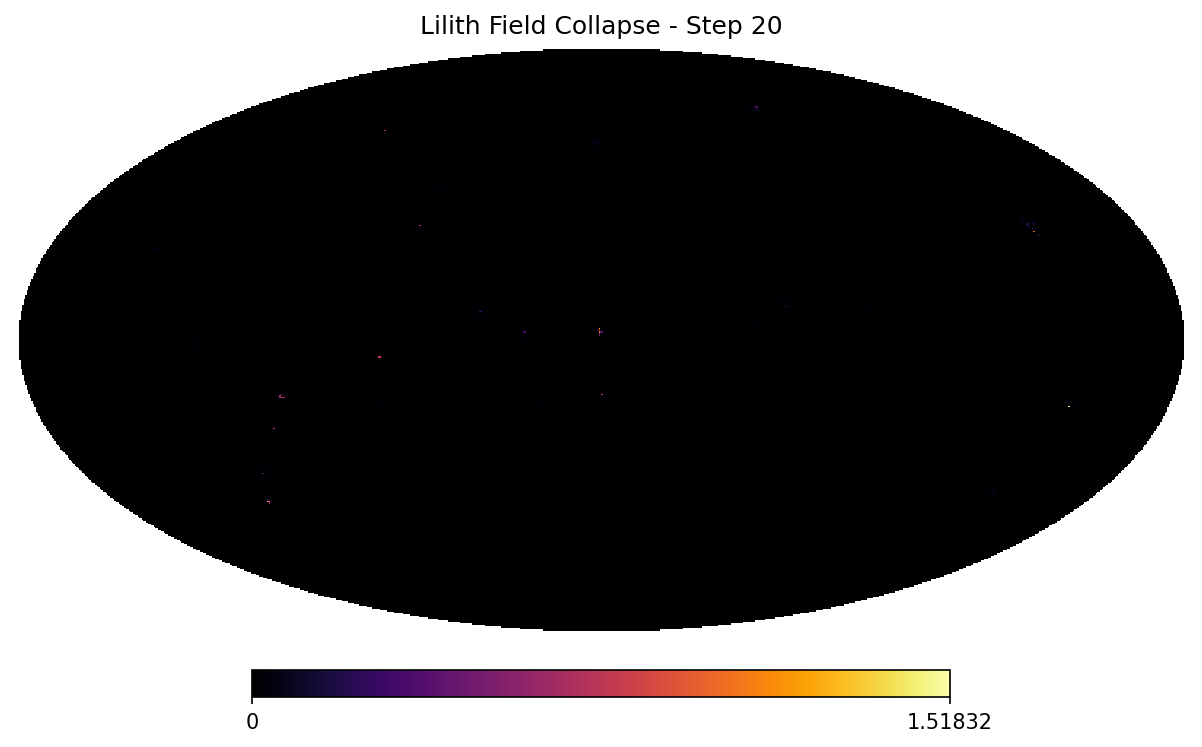
\includegraphics[width=0.45\textwidth]{images/mollweide_000020.png}
  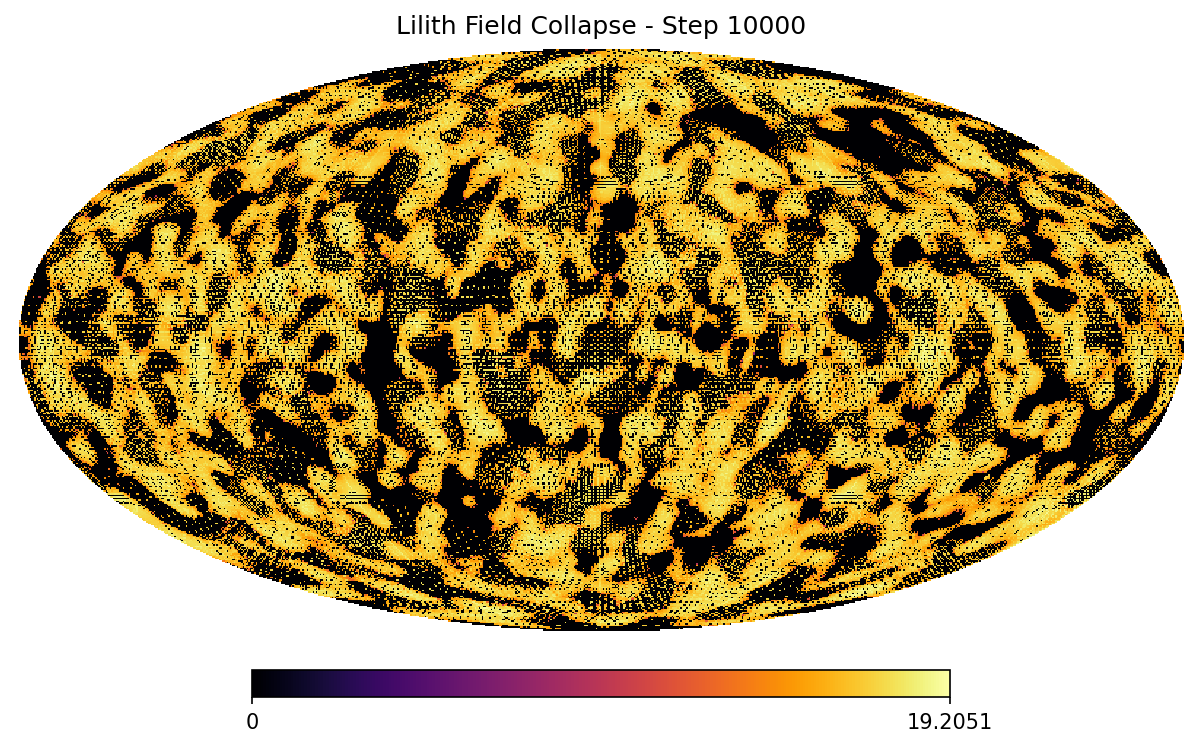
\includegraphics[width=0.45\textwidth]{images/mollweide_010000.png}
  \caption{Mollweide projections of collapse shells at early and late simulation steps.}
\end{figure}

\subsection{Spectral Analysis}
Projected boundary fields are mapped to spherical harmonics via HEALPix, producing $C_\ell$ angular power spectra. These are compared to Planck 2018 spectra using KL divergence, entropy, and correlation metrics.

\begin{figure}[ht]
  \centering
  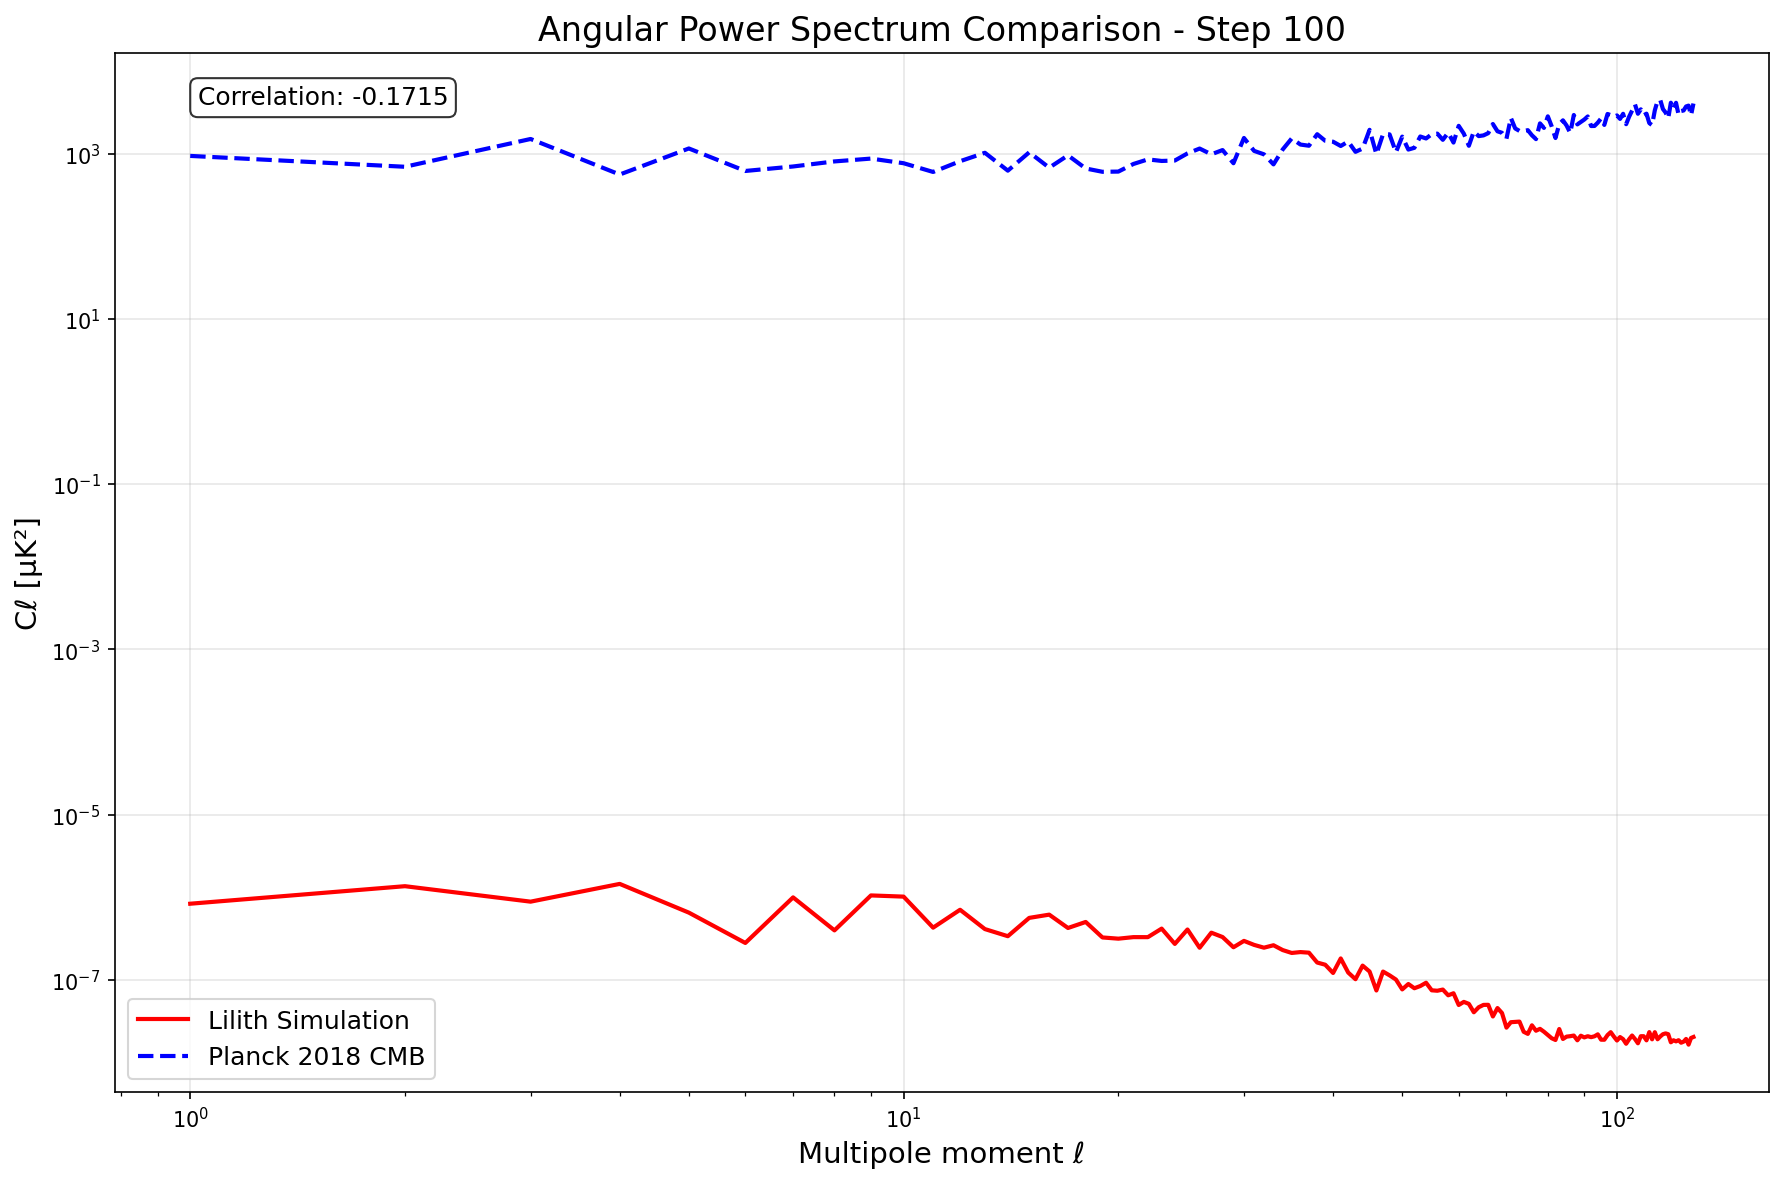
\includegraphics[width=0.9\textwidth]{images/power_spectrum_000100.png}
  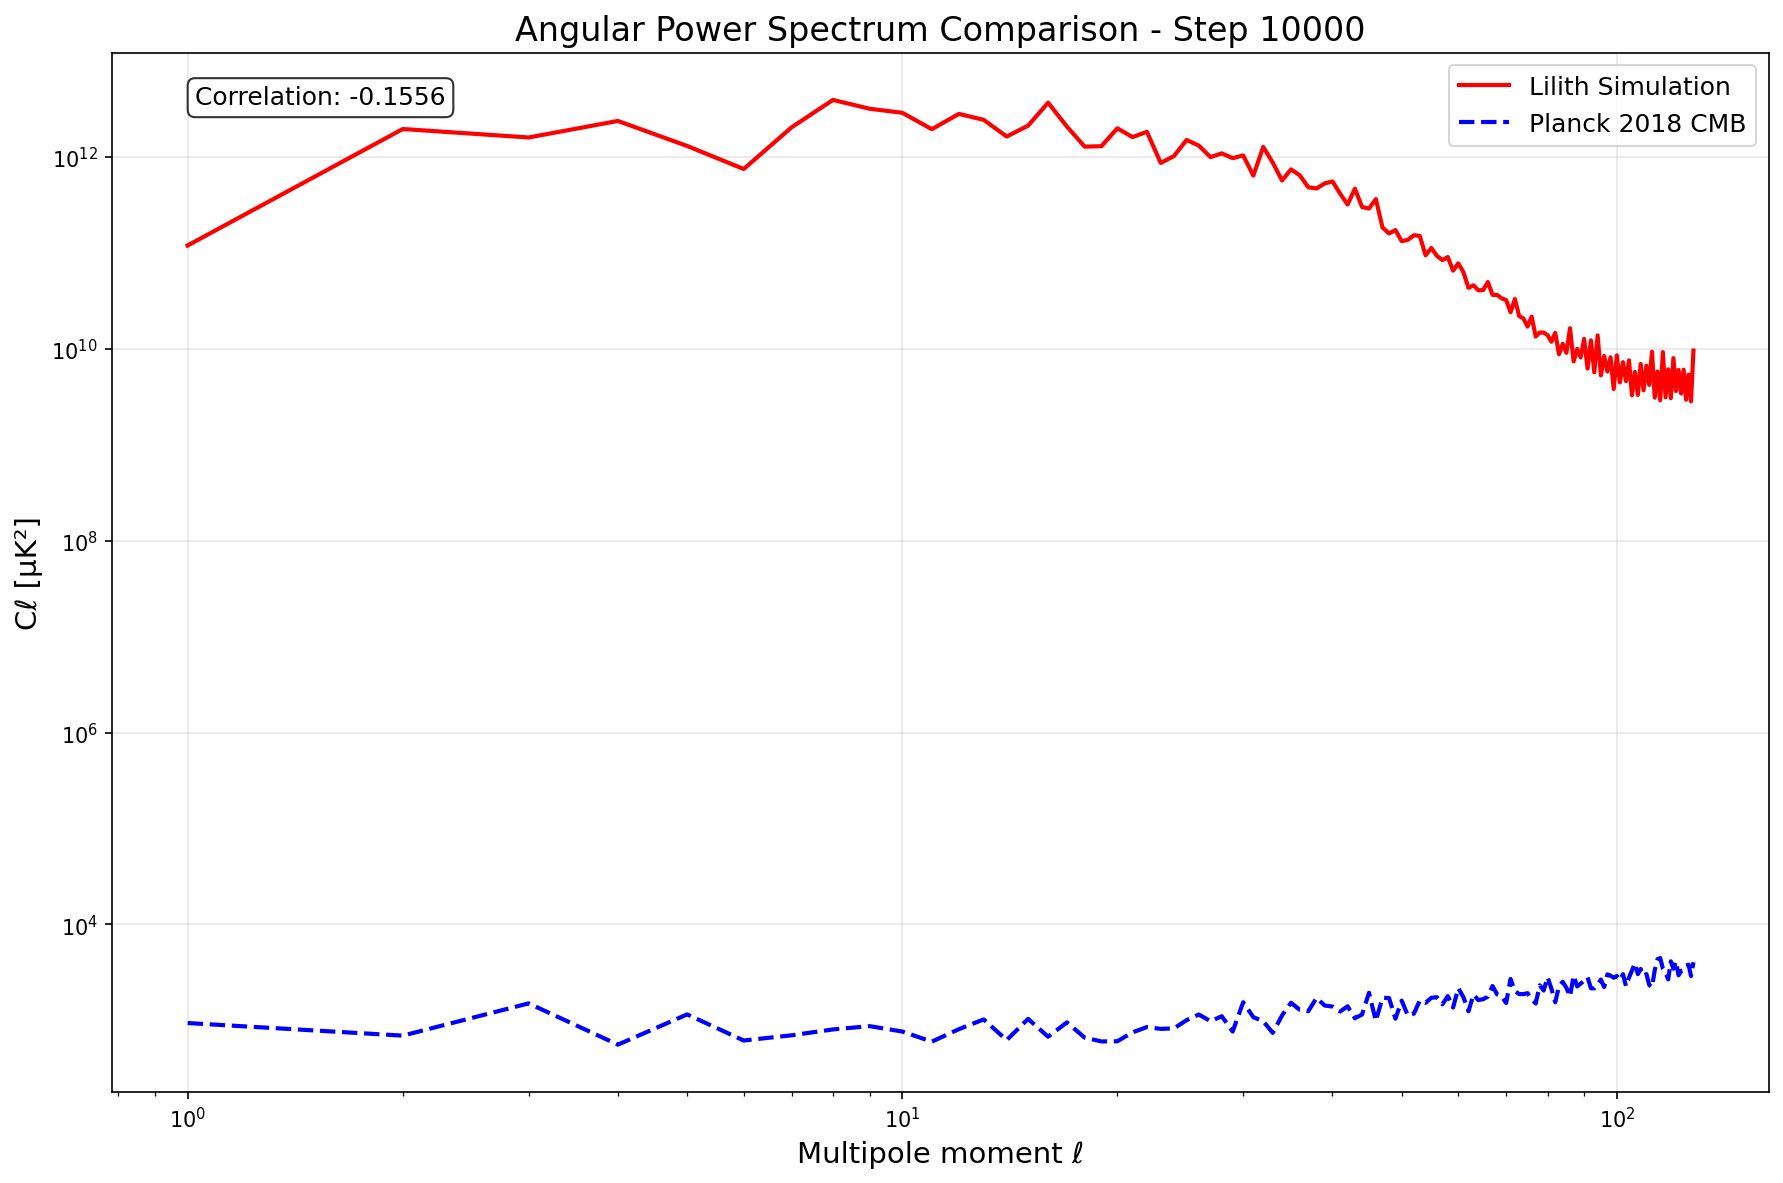
\includegraphics[width=0.9\textwidth]{images/power_spectrum_010000.png}
  \caption{Angular power spectra from shell projections, step 100 (top) and step 10000 (bottom). Note the power level inversion at the early steps after filament and void formation is seen- this is expected behavior considering the long time between genesis and the decay of potential in the CMB at roughly 360000 years after the big bang.}
\end{figure}


\subsection{Conclusion}
Lilith demonstrates that recursive observer-field interaction can yield structured collapse patterns, shell morphogenesis, and measurable angular signatures. Collapse is not symbolic-it is numerically manifest, recursively emergent, and spectrally visible.

\textbf{Lilith does not simulate reality. She asks it to define itself.}


\nocite{*}


\printbibliography

\vspace{2cm}
\begin{center}
    \textcopyright{}
    2025 Ryan Luke Russell. Licensed under CC BY 4.0.
\end{center}


\end{document}